\documentclass[14pt]{extbook}
\usepackage{multicol, enumerate, enumitem, hyperref, color, soul, setspace, parskip, fancyhdr} %General Packages
\usepackage{amssymb, amsthm, amsmath, bbm, latexsym, units, mathtools} %Math Packages
\everymath{\displaystyle} %All math in Display Style
% Packages with additional options
\usepackage[headsep=0.5cm,headheight=12pt, left=1 in,right= 1 in,top= 1 in,bottom= 1 in]{geometry}
\usepackage[usenames,dvipsnames]{xcolor}
\usepackage{dashrule}  % Package to use the command below to create lines between items
\newcommand{\litem}[1]{\item#1\hspace*{-1cm}\rule{\textwidth}{0.4pt}}
\pagestyle{fancy}
\lhead{Progress Quiz 1}
\chead{}
\rhead{Version B}
\lfoot{1269-8776}
\cfoot{}
\rfoot{Fall 2020}
\begin{document}

\begin{enumerate}
\litem{
Write the equation of the line in the graph below in Standard form $Ax+By=C$. Then, choose the intervals that contain $A, B, \text{ and } C$.
\begin{center}
    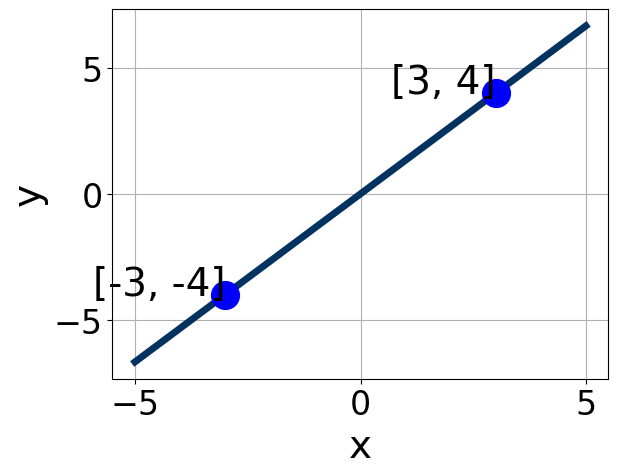
\includegraphics[width=0.5\textwidth]{../Figures/linearGraphToStandardB.png}
\end{center}
\begin{enumerate}[label=\Alph*.]
\item \( A \in [2.3, 4.7], \hspace{3mm} B \in [0.74, 1.41], \text{ and } \hspace{3mm} C \in [-4, -3] \)
\item \( A \in [-5.6, -3.1], \hspace{3mm} B \in [-3.31, -1.28], \text{ and } \hspace{3mm} C \in [6, 14] \)
\item \( A \in [4.8, 5.4], \hspace{3mm} B \in [-3.31, -1.28], \text{ and } \hspace{3mm} C \in [6, 14] \)
\item \( A \in [2.3, 4.7], \hspace{3mm} B \in [-1.94, 0.61], \text{ and } \hspace{3mm} C \in [0, 5] \)
\item \( A \in [4.8, 5.4], \hspace{3mm} B \in [1.33, 2.53], \text{ and } \hspace{3mm} C \in [-11, -7] \)

\end{enumerate} }
\litem{
Find the equation of the line described below. Write the linear equation as $ y=mx+b $ and choose the intervals that contain $m$ and $b$.\[ \text{Perpendicular to } 5 x - 7 y = 11 \text{ and passing through the point } (-2, -4). \]\begin{enumerate}[label=\Alph*.]
\item \( m \in [-1.1, 1.2] \hspace*{3mm} b \in [-7.5, -6.5] \)
\item \( m \in [-3.5, -0.9] \hspace*{3mm} b \in [-3.2, -1.4] \)
\item \( m \in [0.6, 3.3] \hspace*{3mm} b \in [-1.5, -0.5] \)
\item \( m \in [-3.5, -0.9] \hspace*{3mm} b \in [-7.5, -6.5] \)
\item \( m \in [-3.5, -0.9] \hspace*{3mm} b \in [6.5, 7.3] \)

\end{enumerate} }
\litem{
First, find the equation of the line containing the two points below. Then, write the equation as $ y=mx+b $ and choose the intervals that contain $m$ and $b$.\[ (-8, 2) \text{ and } (-2, 8) \]\begin{enumerate}[label=\Alph*.]
\item \( m \in [-0.3, 1.8] \hspace*{3mm} b \in [6.3, 13.6] \)
\item \( m \in [-0.3, 1.8] \hspace*{3mm} b \in [6.3, 13.6] \)
\item \( m \in [-5.3, -0.3] \hspace*{3mm} b \in [5.8, 8.6] \)
\item \( m \in [-0.3, 1.8] \hspace*{3mm} b \in [-12.5, -9.6] \)
\item \( m \in [-0.3, 1.8] \hspace*{3mm} b \in [6.3, 13.6] \)

\end{enumerate} }
\litem{
Solve the equation below. Then, choose the interval that contains the solution.\[ -12(9x + 17) = -13(-11x -5) \]\begin{enumerate}[label=\Alph*.]
\item \( x \in [-0.37, 0.24] \)
\item \( x \in [-1.29, -0.14] \)
\item \( x \in [0.49, 0.92] \)
\item \( x \in [-2.85, -2.6] \)
\item \( \text{There are no real solutions.} \)

\end{enumerate} }
\litem{
Solve the linear equation below. Then, choose the interval that contains the solution.\[ \frac{-3x -9}{2} - \frac{-4x + 4}{7} = \frac{-4x -7}{6} \]\begin{enumerate}[label=\Alph*.]
\item \( x \in [-0.22, 1.78] \)
\item \( x \in [-16.91, -12.91] \)
\item \( x \in [-26.91, -20.91] \)
\item \( x \in [-11.55, -7.55] \)
\item \( \text{There are no real solutions.} \)

\end{enumerate} }
\litem{
Write the equation of the line in the graph below in Standard form $Ax+By=C$. Then, choose the intervals that contain $A, B, \text{ and } C$.
\begin{center}
    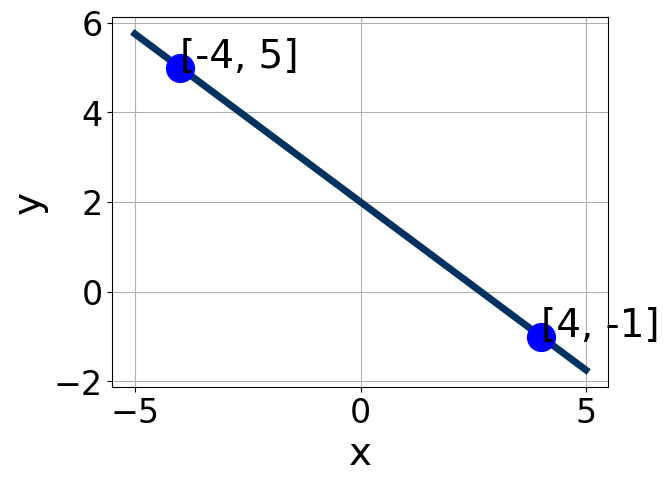
\includegraphics[width=0.5\textwidth]{../Figures/linearGraphToStandardCopyB.png}
\end{center}
\begin{enumerate}[label=\Alph*.]
\item \( A \in [-1.12, 1.47], \hspace{3mm} B \in [-1.81, -0.6], \text{ and } \hspace{3mm} C \in [-3, -1.7] \)
\item \( A \in [1.93, 2.56], \hspace{3mm} B \in [-3.67, -1.36], \text{ and } \hspace{3mm} C \in [-7.4, -5.9] \)
\item \( A \in [-1.12, 1.47], \hspace{3mm} B \in [0.88, 2.07], \text{ and } \hspace{3mm} C \in [1, 5.1] \)
\item \( A \in [-3.16, -1.81], \hspace{3mm} B \in [2.27, 3.47], \text{ and } \hspace{3mm} C \in [5.2, 8.9] \)
\item \( A \in [1.93, 2.56], \hspace{3mm} B \in [2.27, 3.47], \text{ and } \hspace{3mm} C \in [5.2, 8.9] \)

\end{enumerate} }
\litem{
Find the equation of the line described below. Write the linear equation as $ y=mx+b $ and choose the intervals that contain $m$ and $b$.\[ \text{Perpendicular to } 7 x + 4 y = 3 \text{ and passing through the point } (4, -8). \]\begin{enumerate}[label=\Alph*.]
\item \( m \in [0.15, 0.73] \hspace*{3mm} b \in [-11.1, -10.2] \)
\item \( m \in [0.15, 0.73] \hspace*{3mm} b \in [10, 11.4] \)
\item \( m \in [0.15, 0.73] \hspace*{3mm} b \in [-13.1, -11.5] \)
\item \( m \in [-1.23, 0.15] \hspace*{3mm} b \in [-7.1, -4.4] \)
\item \( m \in [1.11, 2.45] \hspace*{3mm} b \in [-11.1, -10.2] \)

\end{enumerate} }
\litem{
First, find the equation of the line containing the two points below. Then, write the equation as $ y=mx+b $ and choose the intervals that contain $m$ and $b$.\[ (-7, 9) \text{ and } (-11, 7) \]\begin{enumerate}[label=\Alph*.]
\item \( m \in [0.4, 2.9] \hspace*{3mm} b \in [17.8, 22.1] \)
\item \( m \in [0.4, 2.9] \hspace*{3mm} b \in [-12.6, -10] \)
\item \( m \in [0.4, 2.9] \hspace*{3mm} b \in [10.8, 13.3] \)
\item \( m \in [-4.8, -0.4] \hspace*{3mm} b \in [0.2, 1.9] \)
\item \( m \in [0.4, 2.9] \hspace*{3mm} b \in [15.3, 16.9] \)

\end{enumerate} }

\litem{
Solve the equation below. Then, choose the interval that contains the solution.\[ -10(5x -8) = -6(-19x -3) \]\begin{enumerate}[label=\Alph*.]
\item \( x \in [-0.44, -0.14] \)
\item \( x \in [-2.51, -1.58] \)
\item \( x \in [-0.15, 0.48] \)
\item \( x \in [-1.34, -0.4] \)
\item \( \text{There are no real solutions.} \)

\end{enumerate} }
\litem{
Solve the linear equation below. Then, choose the interval that contains the solution.\[ \frac{-4x + 7}{6} - \frac{-6x + 9}{2} = \frac{3x + 4}{5} \]\begin{enumerate}[label=\Alph*.]
\item \( x \in [-0.7, 3.2] \)
\item \( x \in [2.4, 4.1] \)
\item \( x \in [-5, -3.8] \)
\item \( x \in [-3.4, -2.1] \)
\item \( \text{There are no real solutions.} \)

\end{enumerate} }
\end{enumerate}

\end{document}